\documentclass[a4paper]{article}
\usepackage{ctex}
%\usepackage{svg}
\usepackage{amssymb,amsmath}
\usepackage{geometry}
\usepackage{graphicx}
\begin{document}
以下的每个魔法题目前面都有标注难度,难度的含义是相对于同类的魔法题目,并不是绝对的难度。
题目中涉及到的几何图形均省略,因为这些图形都很简单,描述起来不会产生歧义。
\section{初中魔法}
\begin{enumerate}
\item (easy)$\triangle ABC$是等腰三角形,而且它可以被分成两个等腰三角形。则$\triangle ABC$
顶角的所有可能值是多少?
\item (easy)现在有足够多的正五边形地砖和正十边形地砖,它们的边长都相等。请问能否用它们覆盖整个平面(地砖之间
不能有重叠)?为什么?
\item (medium)在$\triangle ABC$中,$AD$是$\angle BAC$的平分线,求证:$\frac{AB}{AC}=\frac{BD}{DC}$。
(注:禁止使用相似三角形)。
\item (medium)设函数$y=ax^2+bx+c$的图像如下图。则$b^2-2ac$和$5a^2$的大小关系为?并证明你的结论。
\begin{figure}[!hbp]
\centering
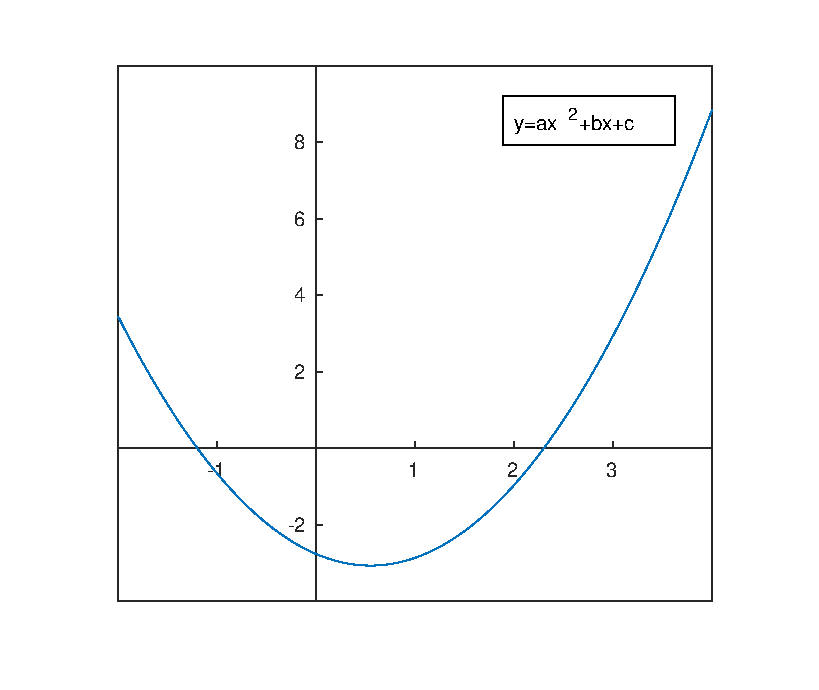
\includegraphics[width=0.5\textwidth]{quad.eps}
\end{figure}
\item (hard)设$\triangle ABC$是等腰三角形,$AB=AC,\angle A=80^\circ$。点$O$为$\triangle ABC$内部
一点,且$\angle OBC=10^\circ,\angle OCA=20^\circ$。求$\angle BAO$的度数。
\end{enumerate}
\section{高中魔法}
\begin{enumerate}
\item (easy)设$a,b,c$是实数,则$a^3+b^3+c^3=3abc$的条件为?
\item (easy)设集合$M=\{1,2\}$,定义集合$A=\{x~|~\forall a \in x, a \in M \}$。则集合$A$和
$M$的关系为?
\item (medium)求值:$\cos\frac{2}{7}\pi+\cos\frac{4}{7}\pi+\cos\frac{6}{7}\pi$
\item (medium)设椭圆$E:\frac{x^2}{a^2}+\frac{y^2}{b^2}=1,a>b>0$,点$P(x_0,y_0)$在椭圆
上。过点$P$分别引出两条斜率为$k_1,k_2$的直线,满足$k_1+k_2=0$。两条直线分别交椭圆于点$A$和$B$。
求证:$AB$的斜率是定值。
\item (hard)设数列$\{a_n\}$满足递推式$a_{n+1}=a_n^2+2,a_0=a$。求$a_n$的表达式。
\end{enumerate}
\section{大学魔法}
\begin{enumerate}
\item (easy)下列说法是否正确?如果正确请证明这个结论,如果不正确请举出反例。
	\begin{enumerate}
	\item 设数列$a_n\rightarrow 0$,$S_n=\sum_{i=1}^{n}a_i$,则$S_n$一定有极限。
	\item 设函数$f(x)$在$\mathbb{R}$上可导,并且有$\lim_{x\rightarrow +\infty}f(x)=0$,
	则有$\lim_{x\rightarrow +\infty}f'(x)=0$。
	\item 可导函数$f(x)$在$\mathbb{R}$上为凸函数当且仅当$f'(x)$是单调递增的。
	\item 设$A\in \mathbb{R}^{n\times n}$,则$A$可以分解为一个对称矩阵和一个反对称矩阵的和。并且这个分解是
	唯一的。
	\end{enumerate}
\item (easy)已知矩阵$A,B$均为半正定矩阵,求证$\mathrm{tr}(AB)\geqslant0$。
\item (medium)设连续函数$f(x)$满足$f(x+y)=f(x)+f(y),\forall x,y \in \mathbb{R}$,求证:
$f(x)=kx$,其中$k\in \mathbb{R}$为一常数。
\item (medium)设矩阵$A$的每个元素为$a_{ij}$,对于任意的$i$,满足$|a_{ii}|>\sum_{j\neq i}{|a_{ji}|}$。
求证:$A$是非奇异矩阵。
\item (medium)设$X$为概率空间$(\Omega,\mathcal{F},P)$上的随机变量,$f(x)$是凸函数。求证:
$f(\mathbb{E}X)\leqslant \mathbb{E}f(X)$,其中$\mathbb{E}(\cdot)$表示对随机变量求期望。
\item (medium)设二元函数$f(x,y)$是凸函数,$C$是凸集。令$g(x)=\inf_{y\in C}f(x,y)$,求证:
$g(x)$为凸函数。
\end{enumerate}
\end{document}